% linux-mcp system architecture (Fig. overview).
% Standalone; compile with: pdflatex linux-mcp-overview.tex
\documentclass[tikz,border=4pt]{standalone}
\usepackage{tikz}
\usepackage{inconsolata}
\usetikzlibrary{positioning,calc,arrows.meta,fit,shapes.geometric,backgrounds}

\definecolor{userBand}{RGB}{247,249,252}
\definecolor{kernBand}{RGB}{240,240,240}
\definecolor{clientFill}{RGB}{230,242,255}
\definecolor{gwFill}{RGB}{255,247,225}
\definecolor{kernFill}{RGB}{232,232,232}
\definecolor{execFill}{RGB}{232,245,233}
\definecolor{sysFill}{RGB}{245,240,252}
\definecolor{edgeDark}{RGB}{70,70,70}

\begin{document}
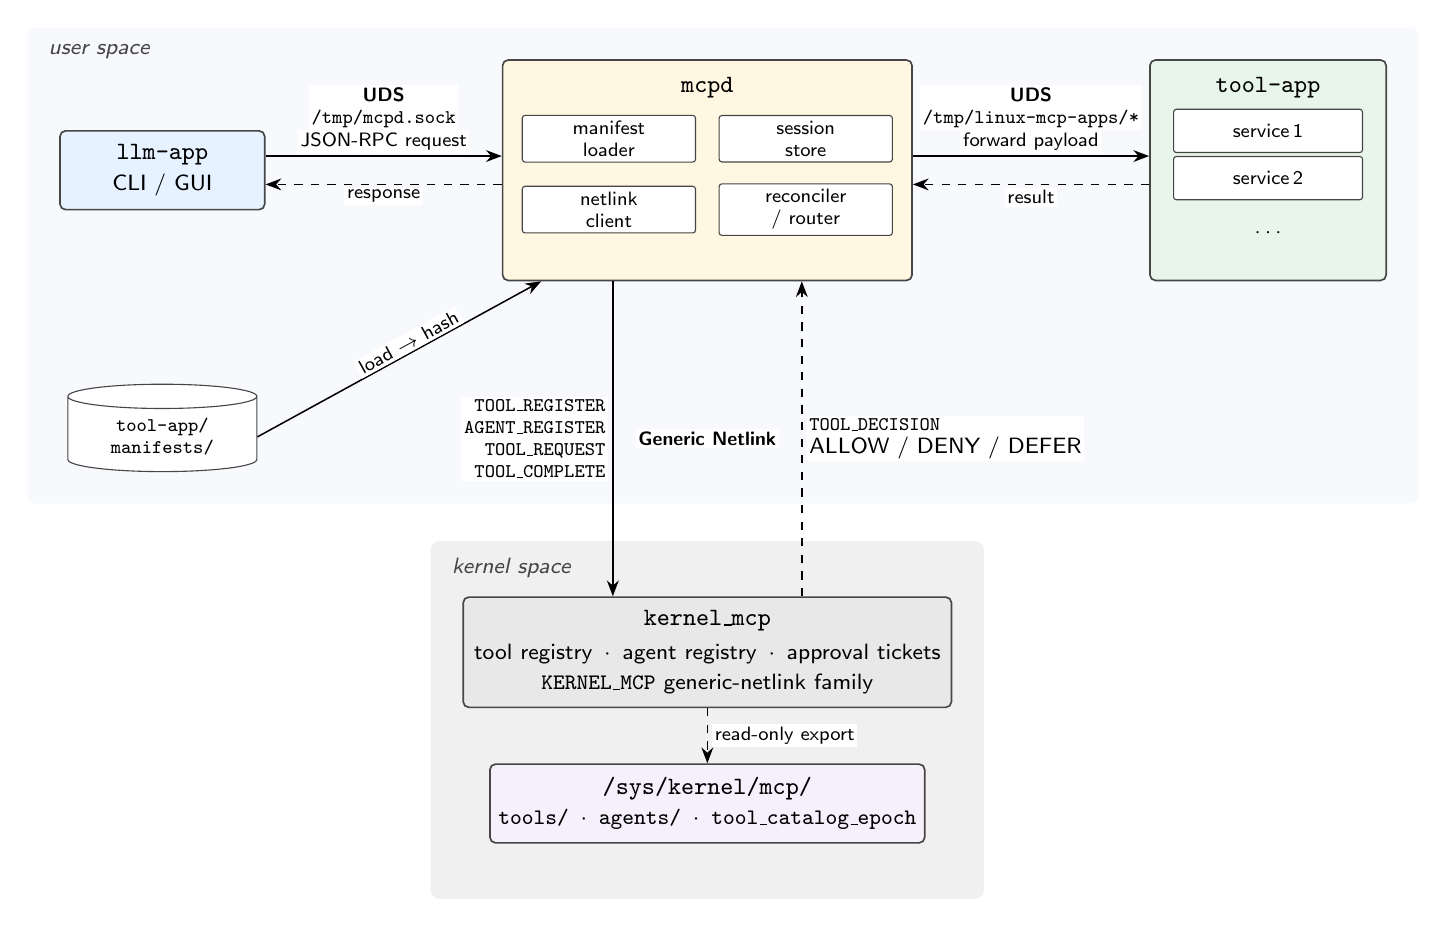
\begin{tikzpicture}[
  font=\small\sffamily,
  comp/.style={draw=edgeDark,rounded corners=2pt,align=center,
               minimum height=10mm,inner sep=3pt,line width=0.6pt},
  sub/.style={draw=edgeDark,rounded corners=1pt,align=center,
              minimum height=5.5mm,inner sep=2pt,
              font=\scriptsize\sffamily,line width=0.4pt,fill=white},
  link/.style={-{Stealth[length=2mm]},line width=0.55pt},
  backlink/.style={-{Stealth[length=2mm]},line width=0.55pt,dashed},
  proto/.style={font=\scriptsize\sffamily,inner sep=1pt,fill=white,align=center},
  band/.style={rounded corners=3pt,inner sep=4mm}
]

% ==========  User-space row  ==========
\node[comp,fill=clientFill,minimum width=26mm] (llm)
  {\texttt{llm-app}\\\footnotesize CLI / GUI};

\node[comp,fill=gwFill,minimum width=52mm,minimum height=28mm,
      right=30mm of llm] (mcpd) {};
\node[anchor=north,font=\small\bfseries,yshift=-1mm] at (mcpd.north) {\texttt{mcpd}};
\node[sub,minimum width=22mm] at ($(mcpd.center)+(-12.5mm, 4mm)$) (ml) {manifest\\loader};
\node[sub,minimum width=22mm] at ($(mcpd.center)+( 12.5mm, 4mm)$) (ss) {session\\store};
\node[sub,minimum width=22mm] at ($(mcpd.center)+(-12.5mm,-5mm)$) (kc) {netlink\\client};
\node[sub,minimum width=22mm] at ($(mcpd.center)+( 12.5mm,-5mm)$) (rt) {reconciler\\/ router};

\node[comp,fill=execFill,minimum width=30mm,minimum height=28mm,
      right=30mm of mcpd] (tool) {};
\node[anchor=north,font=\small\bfseries,yshift=-1mm] at (tool.north) {\texttt{tool-app}};
\node[sub,minimum width=24mm] at ($(tool.center)+(0, 5mm)$)  (t1) {service\,1};
\node[sub,minimum width=24mm] at ($(tool.center)+(0,-1mm)$) (t2) {service\,2};
\node[anchor=center,font=\scriptsize\sffamily] at ($(tool.center)+(0,-8mm)$) {$\cdots$};

% manifests (sits to the LEFT of mcpd, below llm-app height)
\node[cylinder,shape border rotate=90,draw=edgeDark,fill=white,
      aspect=0.2,minimum width=24mm,minimum height=11mm,
      below=22mm of llm,font=\scriptsize\sffamily,align=center] (man)
  {\texttt{tool-app/}\\\texttt{manifests/}};

% ==========  Kernel-space row  ==========
\node[comp,fill=kernFill,minimum width=62mm,minimum height=14mm,
      below=40mm of mcpd] (kern)
  {\texttt{kernel\_mcp}\\[0.3ex]
   \footnotesize tool registry \,$\cdot$\, agent registry \,$\cdot$\, approval tickets\\
   \footnotesize \texttt{KERNEL\_MCP} generic-netlink family};

\node[comp,fill=sysFill,minimum width=52mm,
      below=7mm of kern,align=center] (sysfs)
  {\texttt{/sys/kernel/mcp/}\\
   \footnotesize \texttt{tools/} \,$\cdot$\, \texttt{agents/} \,$\cdot$\, \texttt{tool\_catalog\_epoch}};

% ==========  Bands (background)  ==========
\begin{pgfonlayer}{background}
  \node[band,fill=userBand,fit=(llm)(tool)(mcpd)(man)] (userb) {};
  \node[band,fill=kernBand,fit=(kern)(sysfs),inner ysep=7mm] (kernb) {};
\end{pgfonlayer}
\node[anchor=north west,font=\footnotesize\sffamily\itshape,text=edgeDark]
      at ([xshift=1.5mm,yshift=-1mm]userb.north west) {user space};
\node[anchor=north west,font=\footnotesize\sffamily\itshape,text=edgeDark]
      at ([xshift=1.5mm,yshift=-1mm]kernb.north west) {kernel space};

% ==========  Horizontal arrows  ==========
% llm-app <-> mcpd
\draw[link]     ([yshift= 1.8mm]llm.east)  -- ([yshift= 1.8mm]mcpd.west)
  node[proto,midway,above=0.3mm] {JSON-RPC request};
\draw[backlink] ([yshift=-1.8mm]mcpd.west) -- ([yshift=-1.8mm]llm.east)
  node[proto,midway,below=0.3mm] {response};
\node[proto,above=5mm] at ($(llm.east)!0.5!(mcpd.west)$)
  {\textbf{UDS}\\\texttt{/tmp/mcpd.sock}};

% mcpd <-> tool-app
\draw[link]     ([yshift= 1.8mm]mcpd.east) -- ([yshift= 1.8mm]tool.west)
  node[proto,midway,above=0.3mm] {forward payload};
\draw[backlink] ([yshift=-1.8mm]tool.west) -- ([yshift=-1.8mm]mcpd.east)
  node[proto,midway,below=0.3mm] {result};
\node[proto,above=5mm] at ($(mcpd.east)!0.5!(tool.west)$)
  {\textbf{UDS}\\\texttt{/tmp/linux-mcp-apps/*}};

% manifests -> mcpd (diagonal into mcpd.south west)
\draw[link] (man.east) -- ($(mcpd.south west)+(5mm,0)$)
  node[proto,pos=0.55,above,sloped] {load $\to$ hash};

% ==========  Vertical: mcpd <-> kernel  ==========
% Two parallel arrows separated horizontally with labels on the outside.
% Down arrow (requests) on the LEFT of mcpd's south.
\draw[link]
  ($(mcpd.south)+(-12mm,0)$) -- ($(kern.north)+(-12mm,0)$)
  node[proto,midway,left=0.5mm,align=right]
    {\texttt{TOOL\_REGISTER}\\\texttt{AGENT\_REGISTER}\\\texttt{TOOL\_REQUEST}\\\texttt{TOOL\_COMPLETE}};
% Up arrow (responses) on the RIGHT of mcpd's south.
\draw[backlink]
  ($(kern.north)+(12mm,0)$) -- ($(mcpd.south)+(12mm,0)$)
  node[proto,midway,right=0.5mm,align=left]
    {\texttt{TOOL\_DECISION}\\\footnotesize ALLOW / DENY / DEFER};
% Protocol label between them
\node[proto] at ($(mcpd.south)!0.5!(kern.north)$)
  {\textbf{Generic Netlink}};

% kernel -> sysfs (read-only)
\draw[link,dashed] (kern.south) -- (sysfs.north)
  node[proto,midway,right=0.5mm] {read-only export};

\end{tikzpicture}
\end{document}
